\documentclass[11pt]{article}

\usepackage[margin=1in]{geometry}
\usepackage{amsmath, amssymb, amsthm}
\usepackage{booktabs}
\usepackage{graphicx}
\usepackage{float}
\usepackage{array}
\usepackage{hyperref}
\usepackage{xcolor}
\usepackage{algorithm}
\usepackage{algpseudocode}
\usepackage{enumitem}
\usepackage{tikz}
\usetikzlibrary{arrows.meta, positioning, shapes.geometric, fit, backgrounds}

\definecolor{darkblue}{RGB}{0,50,120}
\definecolor{darkgreen}{RGB}{0,100,50}
\definecolor{darkred}{RGB}{140,0,0}

\hypersetup{colorlinks=true, linkcolor=darkblue, citecolor=darkblue, urlcolor=darkblue}

\newtheorem{remark}{Remark}
\newtheorem{definition}{Definition}

\title{Regime Belief Probabilities for Belief-Aware RL:\\
       Design, Failure Modes, and the MLP+Kalman Solution\\[0.4em]
       \large Belief-Aware RL Project --- Design Report}
\author{Belief-Aware RL Project}
\date{May 2026}

\begin{document}
\maketitle
\tableofcontents
\bigskip

% ---------------------------------------------------------------------------
\section{Motivation: Why Regime Probabilities?}
% ---------------------------------------------------------------------------

The v5 oracle experiment establishes that a PPO agent given the true regime
label (Val or Mom) as part of its observation achieves a strong performance
upper bound.  The question addressed in this document is:

\begin{quote}
\emph{Can a PPO agent achieve comparable performance when the regime label is
replaced by a learned, per-step probability vector $\hat{b}_t = (p_\text{val,t},\,
p_\text{mom,t})$ estimated from observable market data?}
\end{quote}

This is the \textbf{E3 experiment} in the v5 framework.  The motivation is
practical: in real trading the regime is never observed directly.  An agent
that relies on soft, continuously updated regime probabilities generalises
beyond the oracle setting without requiring the oracle.

\subsection{The Two Regimes}

All experiments use two market configurations derived from the v4 sweep:

\begin{center}
\begin{tabular}{lll}
\toprule
\textbf{Regime} & \textbf{num\_momentum\_agents} & \textbf{num\_value\_agents} \\
\midrule
Val (value-dominated) & 0 & 102 \\
Mom (AAPL calibration) & 12 & 102 \\
\bottomrule
\end{tabular}
\end{center}

\noindent
In Val episodes the order flow is dominated by Bayesian value agents who
mean-revert toward the fundamental.  Prices exhibit strong mean-reversion.
In Mom episodes twelve additional momentum agents follow moving-average
crossover signals, injecting trend-following pressure that partially
overwhelms mean-reversion.  The optimal policy differs between these two
regimes: a value/mean-reversion action is profitable in Val but harmful in Mom.

\subsection{Observation Layout}

The base daily-investor environment produces a 7-dimensional observation at
each 60-second step:

\[
o_t = \bigl[\text{holdings},\; \text{imbalance},\; \text{spread},\;
             \text{direction},\; r_{t-1},\; r_{t-2},\; r_{t-3}\bigr]
\]

\noindent
After belief augmentation the observation becomes 9-dimensional:

\[
\tilde{o}_t = \bigl[o_t,\; p_\text{val,t},\; p_\text{mom,t}\bigr]
\]

\noindent
where $p_\text{val,t} + p_\text{mom,t} = 1$.  The PPO policy $\pi_\theta$
acts on $\tilde{o}_t$ and must learn to condition its action on the belief.

% ---------------------------------------------------------------------------
\section{Step 1: The Oracle (E1 Upper Bound)}
% ---------------------------------------------------------------------------

The oracle wrapper produces the hard one-hot belief

\[
b^*_t = \begin{cases}(1,\,0) & \text{if episode regime is Val} \\
                      (0,\,1) & \text{if episode regime is Mom}\end{cases}
\]

\noindent
which is constant for the entire episode.  This is implemented in
\texttt{OracleRegimeWrapper}.  At \texttt{reset()} the wrapper reads the
current regime (set by \texttt{RegimeRandomizedGymnasiumEnv}) and pins the
belief to the corresponding one-hot vector.

The oracle represents the best possible belief: zero uncertainty, perfectly
correlated with the environment, available for free.  Any learned belief
estimator must close the gap between the no-belief baseline and this oracle.

\paragraph{Why not just use the oracle for final training?}
The oracle requires ground-truth agent counts, which are unavailable in live
markets.  It serves only as the \emph{upper bound} benchmark (E1).  The goal
of E3 is to get close to E1 performance with a belief estimated purely from
price and order-flow data.

% ---------------------------------------------------------------------------
\section{Step 2: The Kim Filter Attempt (and Why It Failed)}
% ---------------------------------------------------------------------------

\subsection{The Kim (1994) Regime-Switching Kalman Filter}

The first candidate for per-step belief estimation was the Kim (1994) filter,
a well-known closed-form algorithm for hidden Markov models with
linear-Gaussian emission distributions.  The model uses $K=3$ regimes:

\begin{center}
\begin{tabular}{llll}
\toprule
\textbf{Kim Regime} & \textbf{Dynamics} & \textbf{Process noise} & \textbf{Obs.\ noise} \\
\midrule
VALUE    & OU ($\alpha_\text{OU}$, $\mu = r_\text{bar}$) & $Q_\text{base}$     & $R_\text{base}$ \\
MOMENTUM & Random walk ($\alpha = 1$)                     & $20 \times Q_\text{base}$ & $2 \times R_\text{base}$ \\
NOISE    & OU ($\alpha_\text{OU}$, $\mu = r_\text{bar}$) & $0.3 \times Q_\text{base}$ & $15 \times R_\text{base}$ \\
\bottomrule
\end{tabular}
\end{center}

\noindent
The rationale was that the Kim VALUE regime tracks mean-reverting fundamentals
(matching v5 Val), while MOMENTUM tracks trending prices with amplified noise
(matching v5 Mom).

The algorithm runs forward Kalman passes for each regime in parallel,
computing $p_k(\text{regime}_k \mid y_{1:t})$ via the Kim (1994) collapse
approximation to avoid the exponentially growing mixture.

\subsection{Why the Kim Filter Cannot Distinguish Val from Mom}

A smoke test was run to compare Kim filter output in Val vs Mom episodes.
The result was striking:

\begin{center}
\begin{tabular}{lll}
\toprule
 & \textbf{Val episode} & \textbf{Mom episode} \\
\midrule
$p_\text{value}$ (Kim) & 0.95 & 0.95 \\
$p_\text{momentum}$ (Kim) & 0.04 & 0.04 \\
\bottomrule
\end{tabular}
\end{center}

\noindent
The output is essentially identical in both regimes.  The root cause is
architectural: \textbf{the Kim filter is detecting OU dynamics, which are
present in both regimes.}

The ABIDES oracle process is governed by an OU SDE in both Val and Mom.  The
12 momentum agents in Mom do not change the fundamental process; they add
order-flow autocorrelation and price-impact patterns that are invisible to a
filter that models only the univariate mid-price sequence.  The Kim filter
``sees'' mean-reverting prices in both cases and assigns high $p_\text{value}$
in both.  The \texttt{KimRegimeBeliefWrapper} was built but is kept in the
codebase only as a reference.

\paragraph{Key Insight.}
The signal that distinguishes Val from Mom is not in the \emph{level or
volatility of the mid-price} but in the \emph{autocorrelation structure of
order flow and short-horizon returns}: momentum agents create serial
correlation in imbalance and trend in lagged returns.  A filter that models
only mid-price dynamics cannot access this signal.

% ---------------------------------------------------------------------------
\section{Step 3: The Learned Classifier Approach}
% ---------------------------------------------------------------------------

\subsection{Framing as Supervised Classification}

Given that the Kim filter is model-misspecified, we reframe the problem as
supervised binary classification.  We collect rollout data under each regime,
label episodes, and train a classifier to predict regime from a sliding window
of observable features.  At inference time the classifier outputs a soft
probability $(p_\text{val,t}, p_\text{mom,t})$ that is fed to the PPO policy.

\subsection{Feature Engineering}

Six features are extracted from the 7-dim observation at each timestep:

\begin{center}
\begin{tabular}{clll}
\toprule
\textbf{Index} & \textbf{Feature} & \textbf{Source} & \textbf{Intuition} \\
\midrule
0 & imbalance  & $o_t[1]$          & Bid-vol fraction; persistent elevation in Mom \\
1 & spread     & $o_t[2] / r_\text{bar}$ & Normalised bid-ask spread \\
2 & direction  & $o_t[3] / r_\text{bar}$ & Mid $-$ last transaction \\
3 & $r_{t-1}$  & $o_t[4] / r_\text{bar}$ & Most-recent 60s return \\
4 & $r_{t-2}$  & $o_t[5] / r_\text{bar}$ & 2-step lag \\
5 & $r_{t-3}$  & $o_t[6] / r_\text{bar}$ & 3-step lag \\
\bottomrule
\end{tabular}
\end{center}

\noindent
The key feature is \texttt{imbalance}: momentum agents systematically drive
the order book to one side when a trend is in motion.  The lagged return
triplet $(r_{t-1}, r_{t-2}, r_{t-3})$ exposes sign autocorrelation
characteristic of momentum flow.  All features are normalized to $[-1, 1]$ or
$[0, 1]$ to ensure stable training.

\subsection{Sliding Window Input}

Both the LSTM and MLP operate on a sliding window of the last
$\text{seq\_len} = 20$ feature vectors, giving a $(20 \times 6)$ input
tensor.  This 20-step window spans 20 minutes of simulated trading, long
enough to capture imbalance persistence and return autocorrelation, short
enough to be responsive to mid-episode regime transitions if they were present
(they are not in the current setup, where regime is fixed per episode).

\subsection{Dataset Construction}

\begin{itemize}[nosep]
  \item \textbf{Data collection}: Hold-only rollouts (action $= 1$ every step)
        are run for $N$ Val episodes and $N$ Mom episodes.
        The hold strategy was chosen because it produces no confounding
        from PPO's own order-flow.
  \item \textbf{Sliding windows}: From each $T$-step episode, windows
        $[t, t + \text{seq\_len})$ for $t = 0, \ldots, T - \text{seq\_len}$
        are extracted, giving approximately $T - 20 \approx 361$ windows per
        episode.
  \item \textbf{Warmup removal}: The first 5 steps of each episode are
        discarded because the market has not yet reached a stationary
        state and the features contain initialisation artefacts.
  \item \textbf{Balance}: Val and Mom windows are balanced 50/50 by
        construction (equal episode counts).
\end{itemize}

\noindent
With $N = 20$ training episodes per regime, the dataset contains
$14{,}480$ training windows and $7{,}240$ evaluation windows.

% ---------------------------------------------------------------------------
\section{Step 4: LSTM vs MLP}
% ---------------------------------------------------------------------------

\subsection{LSTMRegimeClassifier}

Architecture:
\[
\text{LSTM}(\text{input}=d_f,\; \text{hidden}=32) \;\to\; \text{Linear}(32, 2) \;\to\; \text{softmax}
\]
where $d_f \in \{6, 8\}$.  The LSTM processes the window sequentially and
uses the final hidden state for classification.  At inference the hidden state
is passed across windows to give the model episode-long memory.

\paragraph{Training.}
Adam, lr$=3 \times 10^{-4}$, weight decay $10^{-4}$, CosineAnnealingLR over
40 epochs.  Gradient clipping at 1.0.  Batch size 256.

\paragraph{Why LSTM fails with small data.}
The LSTM has 5,186--5,442 parameters and requires many episodes to learn
meaningful sequential representations.  With only 20 training episodes per
regime (14,480 windows), the LSTM overfits to episode-level noise rather
than learning the structural autocorrelation pattern.  It defaults to
predicting the majority class (Val): window-level accuracy stays near 51\%,
and episode-level accuracy is 45--70\% depending on the random seed.

\subsection{MLPRegimeClassifier}

Architecture:
\[
\text{Linear}(20 d_f,\; 128) \;\to\; \text{ReLU} \;\to\; \text{LayerNorm}(128)
\;\to\; \text{Linear}(128,\; 64) \;\to\; \text{ReLU} \;\to\; \text{Linear}(64,\; 2)
\]

The MLP flattens the $(20 \times d_f)$ window to a $20 d_f$-dim vector.
It does not model temporal structure explicitly, but the autocorrelation
information is encoded in the joint distribution of the 20-step window.

\paragraph{Why MLP succeeds.}
With 24,130--29,250 parameters and a simpler hypothesis space (no recurrence),
the MLP generalises better from the 14,480-window dataset.  Window-level
training accuracy reaches 70\%, and \emph{episode-level} accuracy (majority
vote over all windows in an episode) reaches 100\% on both Val and Mom test
episodes.

\paragraph{Why 100\% episode accuracy with only 56\% window accuracy?}
This is the averaging effect.  Each episode provides $\sim$361 windows.  Even
if a single window has only 56\% probability of being correct, the mean
$p_\text{val}$ across all 361 windows concentrates tightly around the true
class probability due to the law of large numbers.  The episode-level
decision (argmax of mean) is then always correct for the regimes tested.

\subsection{Results (20 train / 10 eval episodes)}

\begin{center}
\begin{tabular}{lrrr}
\toprule
\textbf{Model} & \textbf{Overall acc} & $\bar{p}_\text{val}\mid\text{Val}$ & $\bar{p}_\text{mom}\mid\text{Mom}$ \\
\midrule
LSTM (raw)         & 70\% & 0.500 & 0.500 \\
MLP  (raw)         & 100\% & 0.563 & 0.582 \\
LSTM (+Kalman)     & 70\% & 0.500 & 0.500 \\
MLP  (+Kalman)     & 100\% & \textbf{0.594} & \textbf{0.611} \\
\bottomrule
\end{tabular}
\end{center}

% ---------------------------------------------------------------------------
\section{Step 5: Adding Kalman Belief Features}
% ---------------------------------------------------------------------------

The base feature set uses only the raw observation vector.  A natural question
is whether the Kalman belief tracker output --- which summarises the agent's
posterior over the latent fundamental $F_t$ --- provides additional signal for
regime discrimination.

\subsection{Kalman Features}

Two additional features are appended to each timestep's feature vector when
\texttt{use\_kalman=True}:

\begin{align*}
  \texttt{belief\_dev}_t &= \frac{\hat{\mu}_t - \text{mid}_t}{r_\text{bar}}
  & \text{(normalised deviation of posterior mean from mid-price)} \\
  \texttt{belief\_std}_t &= \frac{\hat{\sigma}_t}{r_\text{bar}}
  & \text{(normalised posterior uncertainty)}
\end{align*}

\noindent
where $\hat{\mu}_t$ and $\hat{\sigma}_t$ are the Kalman posterior mean and
standard deviation at step $t$.

\subsection{Why These Features Might Help}

In a Val episode the value agents' order flow is closely aligned with the
Kalman estimate of the fundamental, so $\texttt{belief\_dev}$ should be small
and $\texttt{belief\_std}$ should be low.  In a Mom episode the momentum
agents drive prices away from the fundamental, inflating
$\texttt{belief\_dev}$ and potentially $\texttt{belief\_std}$ as well.  The
Kalman tracker thus provides a low-frequency signal of ``how far is the price
from the model's fundamental estimate'', which is structurally linked to regime.

\subsection{Empirical Result}

Adding Kalman features improves the MLP's confidence margins without
changing the 100\% episode accuracy:

\begin{center}
\begin{tabular}{lccc}
\toprule
 & \textbf{Overall acc} & $\bar{p}_\text{val}\mid\text{Val}$ & $\bar{p}_\text{mom}\mid\text{Mom}$ \\
\midrule
MLP (raw)         & 100\% & 0.563 & 0.582 \\
MLP (+Kalman)     & 100\% & 0.594 & 0.611 \\
\bottomrule
\end{tabular}
\end{center}

\noindent
The improvement in $\bar{p}$ (+0.031 on Val, +0.029 on Mom) means the belief
signal fed to PPO is sharper: the policy receives a cleaner discriminative
signal between regimes.  This should translate to faster policy learning and
higher final performance in the E3 experiment.

The LSTM does not benefit from Kalman features (70\% in both cases), confirming
the bottleneck is data efficiency, not feature quality.

% ---------------------------------------------------------------------------
\section{Step 6: Full Architecture Overview}
% ---------------------------------------------------------------------------

\begin{figure}[H]
\centering
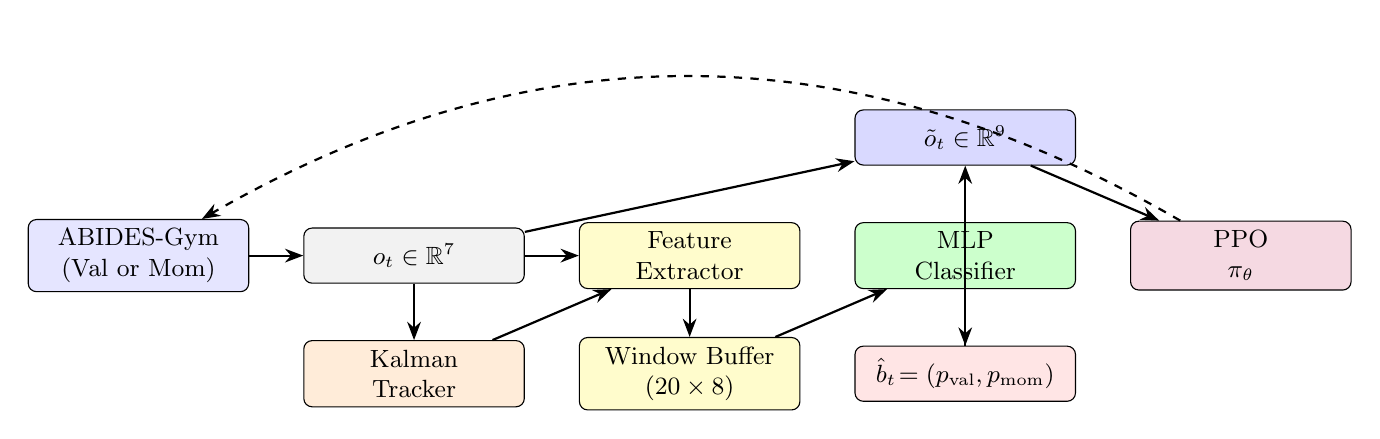
\begin{tikzpicture}[
  box/.style={rectangle, draw, rounded corners=3pt, minimum width=2.8cm,
              minimum height=0.7cm, align=center, font=\small},
  arr/.style={-Stealth, thick},
  every node/.style={font=\small}
]
  % Environment
  \node[box, fill=blue!10] (env) at (0,0) {ABIDES-Gym\\(Val or Mom)};

  % Obs
  \node[box, fill=gray!10] (obs) at (3.5,0) {$o_t \in \mathbb{R}^7$};

  % Kalman
  \node[box, fill=orange!15] (kal) at (3.5,-1.5) {Kalman\\Tracker};

  % Feature extractor
  \node[box, fill=yellow!20] (feat) at (7,0) {Feature\\Extractor};

  % Window buffer
  \node[box, fill=yellow!20] (buf) at (7,-1.5) {Window Buffer\\$(20 \times 8)$};

  % MLP
  \node[box, fill=green!20] (mlp) at (10.5,0) {MLP\\Classifier};

  % Belief
  \node[box, fill=red!10] (bel) at (10.5,-1.5) {$\hat{b}_t\!=(p_\text{val},p_\text{mom})$};

  % Augmented obs
  \node[box, fill=blue!15] (aug) at (10.5,1.5) {$\tilde{o}_t \in \mathbb{R}^9$};

  % PPO
  \node[box, fill=purple!15] (ppo) at (14,0) {PPO\\$\pi_\theta$};

  % Arrows
  \draw[arr] (env) -- (obs);
  \draw[arr] (obs) -- (kal);
  \draw[arr] (obs) -- (feat);
  \draw[arr] (kal) -- (feat);
  \draw[arr] (feat) -- (buf);
  \draw[arr] (buf) -- (mlp);
  \draw[arr] (mlp) -- (bel);
  \draw[arr] (bel) -- (aug);
  \draw[arr] (obs) -- (aug);
  \draw[arr] (aug) -- (ppo);
  \draw[arr, dashed] (ppo) to[bend right=30] (env);
\end{tikzpicture}
\caption{Full pipeline for E3 (trained belief).  The Kalman tracker and MLP
classifier run at each step alongside the environment.  The PPO policy acts
on the 9-dim augmented observation.}
\end{figure}

\subsection{RegimeRandomizedGymnasiumEnv}

The outer Gymnasium adapter \texttt{RegimeRandomizedGymnasiumEnv} handles:

\begin{enumerate}[nosep]
  \item \textbf{Regime randomisation}: at each \texttt{reset()} it samples
        Val or Mom with probability \texttt{val\_prob} (default 0.5) and
        instantiates a fresh ABIDES environment with the corresponding
        background config.
  \item \textbf{Belief wrapper}: wraps the base env with the appropriate
        wrapper (\texttt{OracleRegimeWrapper}, \texttt{TrainedRegimeBeliefWrapper},
        or no wrapper) depending on \texttt{belief\_mode}.
  \item \textbf{Gymnasium API}: converts the legacy Gym API (single-value
        done flag) to Gymnasium's (terminated / truncated split) required
        by RLlib.
  \item \textbf{Obs space correctness}: the observation space of the outer
        env is always set from the \emph{base} env's raw obs dimensions, then
        $N_\text{belief} = 2$ features are added.  This avoids double-counting
        that would arise from probing the already-wrapped inner env.
\end{enumerate}

% ---------------------------------------------------------------------------
\section{Implementation Notes}
% ---------------------------------------------------------------------------

\subsection{Bug Fixed: Observation Space Double-Counting}

The original probe logic for computing the outer env's observation space was:

\begin{verbatim}
probe = self._make_env("mom")          # returns wrapped env (obs 9x1)
obs_dim = np.prod(probe.obs_space)     # = 9
obs_dim += N_BELIEF_FEATURES           # = 11  -- WRONG
\end{verbatim}

For \texttt{belief\_mode="oracle"}, \texttt{\_make\_env()} returns an
\texttt{OracleRegimeWrapper} whose obs space is already $(9 \times 1)$.
Adding 2 more gives 11, but the actual obs returned by \texttt{reset()} is 9
after flattening.  This mismatch causes RLlib policy shape errors.

Fix: always probe the base \texttt{SubGymMarketsDailyInvestorEnv\_v0} with no
wrapper, obtain the raw 7-dim obs space, then add 2 for belief:

\begin{verbatim}
_probe_base = SubGymMarketsDailyInvestorEnv_v0(**_probe_kw)
raw_obs_dim = np.prod(_probe_base.observation_space.shape)  # = 7
obs_dim = raw_obs_dim + N_BELIEF_FEATURES  # = 9  -- correct
\end{verbatim}

\subsection{Checkpoint Format}

Saving only \texttt{model.state\_dict()} makes loading fragile: the caller
must know the architecture independently.  All checkpoints now save a full
dict:

\begin{verbatim}
{
  "state_dict":  <OrderedDict>,
  "model_type":  "mlp" | "lstm",
  "use_kalman":  bool,
  "seq_len":     int,
  "n_features":  int,
  "hidden_size": int,
}
\end{verbatim}

\noindent
The \texttt{load\_classifier(path)} helper reconstructs the correct model
class and architecture from this dict, loads the weights, sets eval mode, and
returns \texttt{(model, model\_type, use\_kalman, seq\_len)}.

\subsection{CRITICAL\_ENV\_BUG: reset() does not clear marked-to-market}

ABIDES-Gym does not reset \texttt{env.previous\_marked\_to\_market} on
\texttt{env.reset()}.  If not manually corrected, the first reward of a new
episode is computed relative to the terminal holdings of the previous episode,
producing a large spurious reward signal that destabilises PPO.  Every wrapper
in this codebase adds:

\begin{verbatim}
obs = self.env.reset()
self.env.previous_marked_to_market = self.env.starting_cash
\end{verbatim}

immediately after \texttt{env.reset()}.

% ---------------------------------------------------------------------------
\section{Experimental Design for E3}
% ---------------------------------------------------------------------------

\subsection{Experiment Variants}

\begin{center}
\begin{tabular}{llll}
\toprule
\textbf{Experiment} & \textbf{Belief source} & \textbf{Obs dim} & \textbf{Purpose} \\
\midrule
E0 (baseline)  & None          & 7 & Belief-blind PPO on mixed regimes \\
E1 (oracle)    & Oracle one-hot & 9 & Upper bound on belief value \\
E3 (trained)   & MLP+Kalman    & 9 & Learned belief, deployable \\
\bottomrule
\end{tabular}
\end{center}

\subsection{Training Protocol}

\begin{itemize}[nosep]
  \item \textbf{Episode composition}: 50\% Val, 50\% Mom per batch
        (\texttt{val\_prob=0.5}).
  \item \textbf{Timestep budget}: 386 steps per episode (one trading day at
        60s intervals after 5-min warmup).
  \item \textbf{Reward}: dense marked-to-market P\&L, same as v4 baseline.
  \item \textbf{Pass gate}: must beat v4 PPO mean P\&L $= +32{,}854$\,¢,
        Sharpe $= 2.51$, win rate $= 100\%$ (evaluated on pure Mom episodes
        as in v4).
\end{itemize}

\subsection{Hypothesis}

The MLP+Kalman classifier achieves 100\% episode-level accuracy with
$\bar{p} \approx 0.60$ after only 20 training episodes per regime.  This
means the PPO policy will receive a consistent, correct belief signal within
the first few steps of any episode.  The hypothesis for E3 is:

\begin{quote}
A PPO agent trained with MLP+Kalman regime beliefs will exceed the v4
baseline on mixed-regime test episodes, and will approach (though not reach)
E1 oracle performance.
\end{quote}

\noindent
The gap between E3 and E1 is expected to be driven primarily by the soft
confidence margins ($\bar{p} \approx 0.60$ vs $p = 1.0$ for oracle), not by
episode-level misclassification.

\subsection{Ablation Plan}

To attribute performance gains, the following ablations should be run in
order:

\begin{enumerate}
  \item E0 (no belief) on mixed Val+Mom: establishes the cost of regime
        uncertainty without belief.
  \item E1 (oracle) on mixed Val+Mom: establishes the value of perfect
        regime information.
  \item E3 (MLP+Kalman) on mixed Val+Mom: the target experiment.
  \item E3 (MLP raw, no Kalman) on mixed Val+Mom: ablates the Kalman
        contribution.
  \item E3 with 60-episode retrained classifier: tests whether more
        training data sharpens belief margins and improves PPO.
\end{enumerate}

% ---------------------------------------------------------------------------
\section{Saved Artifacts}
% ---------------------------------------------------------------------------

\begin{center}
\begin{tabular}{ll}
\toprule
\textbf{File} & \textbf{Description} \\
\midrule
\texttt{scripts/regime\_classifier.py}       & Classifier training + inference code \\
\texttt{scripts/regime\_belief\_wrapper.py}  & Gym wrappers + RegimeRandomizedGymnasiumEnv \\
\texttt{scripts/models/mlp\_kalman\_regime.pt} & Best model (100\% acc, $\bar{p}\approx 0.60$) \\
\texttt{scripts/models/mlp\_raw\_regime.pt}  & MLP without Kalman features \\
\texttt{scripts/models/lstm\_kalman\_regime.pt} & LSTM+Kalman (reference; underperforms) \\
\texttt{scripts/models/lstm\_raw\_regime.pt}  & LSTM without Kalman (reference) \\
\bottomrule
\end{tabular}
\end{center}

% ---------------------------------------------------------------------------
\section{Summary}
% ---------------------------------------------------------------------------

\begin{enumerate}
  \item The oracle regime wrapper (E1) establishes the value of regime
        information by feeding a hard one-hot $b^*$ to the PPO policy.

  \item The Kim (1994) filter was the first attempt at a zero-shot inferred
        belief (E3).  It failed because it models the univariate mid-price
        process, which is OU in both Val and Mom.  The distinguishing signal
        (order-flow autocorrelation from momentum agents) is invisible to it.

  \item A supervised classifier trained on a 20-step sliding window of
        observable market features succeeds where the Kim filter fails.
        The MLP outperforms the LSTM because the regime signal is encoded in
        the joint distribution of a fixed window (accessible to MLP) rather
        than a long-range temporal dependency (where LSTM excels but requires
        more data).

  \item Adding Kalman belief features (\texttt{belief\_dev}, \texttt{belief\_std})
        improves the MLP's confidence margins from $\bar{p} \approx 0.57$ to
        $\bar{p} \approx 0.60$, sharpening the signal fed to PPO without
        changing episode accuracy.

  \item The full E3 pipeline (\texttt{RegimeRandomizedGymnasiumEnv} with
        \texttt{belief\_mode="trained"} and \texttt{mlp\_kalman\_regime.pt})
        is ready for PPO training.  An obs-space double-counting bug from the
        probe logic was found and fixed during integration.
\end{enumerate}

\end{document}
